\Chapter{Javító Szoftver Megvalósítás}
A szoftver egy C nyelvű csomagként került megvalósításra, obj\_corrector\_tool (Objektum Javító Eszköz) névvel ellátva. A mappa tartalmazza az összes fájl-t a programhoz illetve az egységtesztekhez.\\

Csomag struktúrális felépítése a következő:
\bigskip
\dirtree{%
.1 /obj\_corrector\_tool.
.2 /include.
.3 bounding\_box.h.
.3 draw.h.
.3 model.h.
.3 \ldots.
.2 /OBJ.
.3 bird.
.4 bird.jpg.
.4 bird.obj.
.4 bird.mtl.
.4 \ldots.
.3 cube.
.4 cube.png.
.4 cube.obj.
.4 cube.mtl.
.3 \ldots.
.2 src.
.3 bounding\_box.c.
.3 draw.c.
.3 model.c.
.3 main.c.
.3 \ldots.
.2 tests.
.3 regex\_tests.h.
.3 test\_runner.c.
.2 Makefile.
}
\newpage
\texttt{Include} mappa tartalmazza a szükséges header állományokat.  \texttt{OBJ} almappáiban találhatóak a felhasznált OBJ fájlok. Az \texttt{src}-ben találhatóak a C nyelvű programfájlok. \texttt{Tests} mappában található Cmockában írt egységtesztek . Végül közvetlen az \texttt{obj\_\\corrector\_tool} található a \texttt{Makefile} .\\

\Section {Funkció hívás diagram}
\begin{figure}[h]
\centering
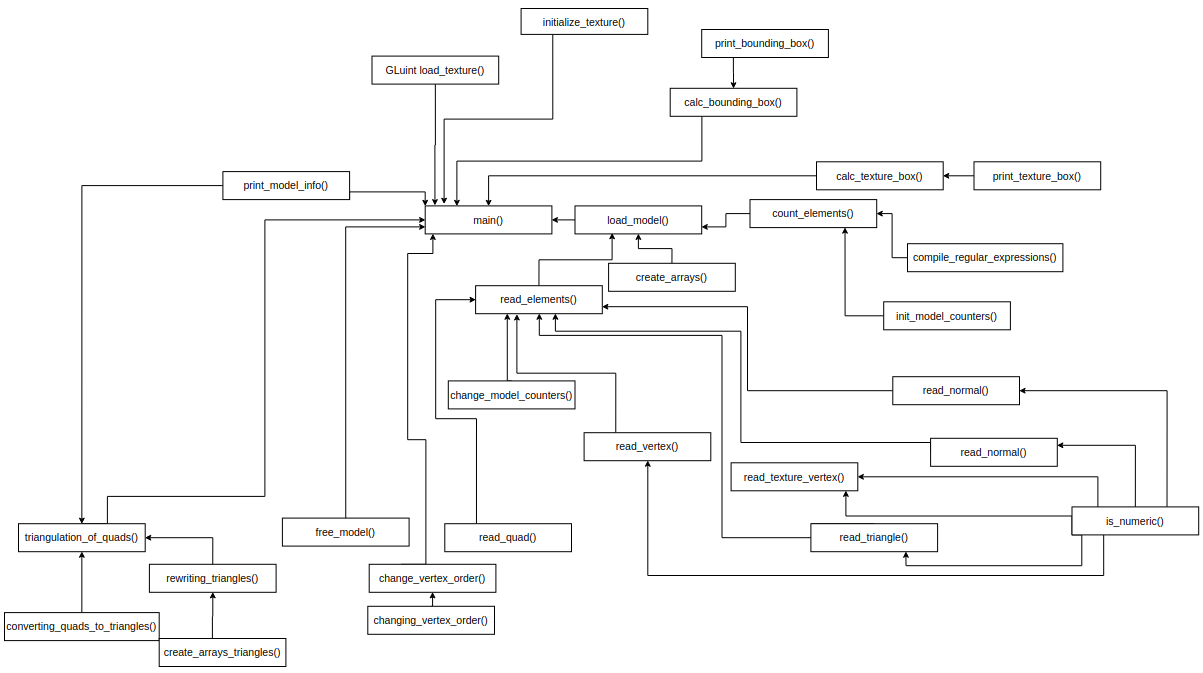
\includegraphics[width=\textwidth]{images/func.png}
\caption{Teljes Funkcióhívás Diagram.}
\label{fig:funk}
\end{figure}

\Aref{fig:funk} diagramon látható a program teljes funkcióhívás diagramja. Ez a diagram nagyon komplex és rengetek különálló funkciót kezel egyben. A különböző függvények egymást hívják meg a program futattása során végül az összes főbb funkció a \texttt{main} funkcióban találkozik.\\

Értelemszerűen, hogy egy OBJ javító alkalmazásról lévén szó az egyes funkciókat érdemes együtt  kezelni\\

Program főbb funkciói:
 \begin{itemize}
\item modell beolvasás
\item textúra beolvasás
\item hibák javítása
\item fájlba írás
\item megjelenítés
\end{itemize}
\bigskip
Feldolgozási folyamatot fentről-lefelé értelmezhetjük.
\newpage
\Section {Modell Beolvasás}
Az alkalmazás minden olyan OBJ fájl betöltésére alkalmas, ami nem tartalmaz négyszögnél nagyobb csúcsszámmal rendelkező síkodomot, amennyiben az OBJ fájlunk tartalmaz ennél magasabb számút, azok számát képes összeszámlálni, viszont kezelni nem.\\

Elemzésre és javításra szánt OBJ fájl betöltése \texttt{main.c} (C nyelven írt programfájlon) belül \texttt{load\_model} függvénnyel történhet:
\bigskip
\begin{cpp}
load_model("utvonal/pelda.kiterjesztes", &model, &regular);
\end{cpp}
\bigskip

\texttt{utvonal}nál meg kell adni a fájl elérési útvonalát, majd a \texttt{pelda} helyére az \texttt{OBJ} fájlunk nevét majd a kiterjesztést (\texttt{.obj}).
\bigskip

\noindent Modell struktúra feltöltés bemutatása funkcióhívásokkal:\\

\texttt{Load\_model} beolvassa a megadott \texttt{OBJ} fájlt.
\begin{figure}[h]
\centering
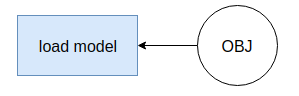
\includegraphics[scale=0.5]{images/load.png}
\end{figure}
\bigskip

Beolvasás után \texttt{count\_elements} összeszámolja \texttt{model} struktúra \texttt{n\_vertices},  \texttt{\\n\_texture\_vertices}, \texttt{n\_normals}, \texttt{n\_faces} illetve \texttt{n\_triangles}, \texttt{n\_quads} és \texttt{n\\\_polygons} egyes értékeit.
\begin{figure}[h]
\centering
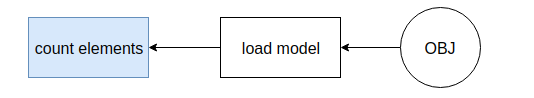
\includegraphics[scale=0.5]{images/count.png}
\end{figure}
\bigskip

Majd az összeszámolt értékek számával \texttt{create\_arrays} lefoglalja a szükséges nagyságú tömböket.
\begin{figure}[h]
\centering
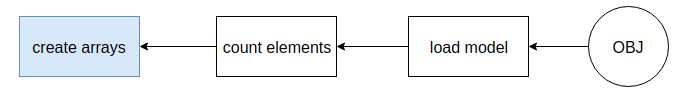
\includegraphics[scale=0.5]{images/create.png}
\end{figure}
\bigskip
\newpage
Ezután lefoglalt tömböt  a \texttt{read\_elements} kiolvassa a fájlból és feltölti az egyes értékekkel.
\begin{figure}[h]
\centering
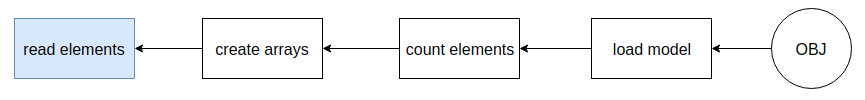
\includegraphics[scale=0.5]{images/read.png}
\end{figure}
\Section {Textúra}
Textúra pontok \texttt{u}, \texttt{v} [0 ; 1] intervallumon belül kell elhelyezkedni,ez az OBJ fájlok egy részében nem ígyvan ennek ellenőrzésére  a  \texttt{print\_texture\_box} nyújthat segítséget. Amennyiben utasítjuk a programot  a texture\_box kiszámítására és megjelenítésére, abban az esetben egy fix struktúrát jelenít meg számunkra a program és benne jelzi a számított adatokat.
\begin{python}
Texture box:
u in [0.000000, 1.000000]
v in [0.000000, 1.000000]
\end{python}

Balról jobbra haladva először megjeleníti a fájlban \textbf{u} legkisebb és legnagyobb értékét, majd ugyanezt megcsinálja a \textbf{v} koordináta számított adataival is.\\

Szoftver 2D (kép formátumú) textúrák megjelenítését támogatja  kívánt fájl megadása \texttt{texture.c} programfájlon belül \texttt{texture\_filename} után lehetséges.
\bigskip
\begin{cpp}
char texture_filename[] = "utvonal/pelda.kiterjesztes";
\end{cpp}
\bigskip

Saját képfájlunk megadásánál \texttt{utvonal} helyére a fájlunk elérési útvonala \texttt{pelda} helyére a képfájlunk neve \texttt{kiterjesztes} helyére pedig kiterjesztés kerül (\texttt{.jpg , .png, .tga}).
\Section {Megjelenítés}
Modellek mérete és elhelyezkedése nagy mértékben eltérő lehet. Ennek elemzése érdekében érdemes megnézni a \texttt{print\_bounding\_box} által számított adatokat és a kamerát ennek megfelelően pozíciónálni.
\bigskip
\begin{python}
Bounding box:
x in [-0.500000, 0.500000]
y in [-0.500000, 0.500000]
z in [-0.500000, 0.500000]
\end{python}
\bigskip

Ezen számok megadják, hogy az OBJ fájlunk mérete mekkora lesz a térben. Minden koordináta első száma a legkisebb második száma pedig a legnagyobb csúcs értékének elhelyezkedését adja az adott síkon.
\bigskip
\begin{cpp}
gluLookAt
(
        0.0, 0.0, -200, //eye (X, Y, Z)
        0.0, 0.0, 0.0,  //center (X, Y, Z)
        0.0, 1.0, 0.0 //up (X, Y, Z)
);
\end{cpp}
\bigskip

Kamera pozíciót a \texttt{gluLookAt} paraméterei állításával lehet pozícionálni.\\

Javító szoftver lévén maga a megjelenítő minimális funkciókkal lett ellátva, tehát nem tudjuk mozgatni  a modellünket, illetve kamera pozíciója sem változtatható megjelenítés után. Egyedül a modell forgatása lehetséges egér segítségével.\\

\texttt{house.obj} megjelenítése a hozzátartozó textúrával.(\ref{fig:demo} ábra)
\bigskip

\begin{figure}[h]
\centering
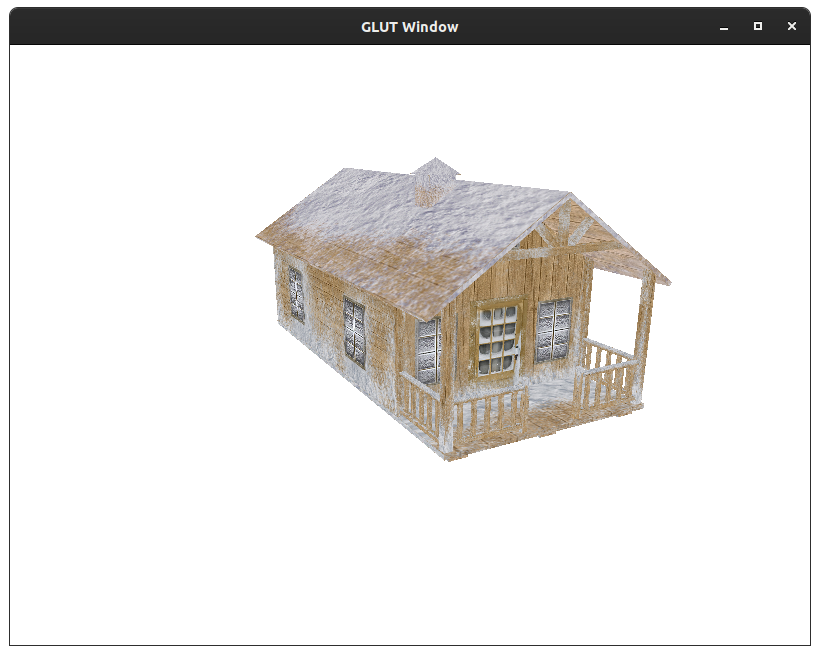
\includegraphics[width=\textwidth]{images/demo.png}
\caption{House modell megjelenítés.}
\label{fig:demo}
\end{figure}
\newpage
\Section {Javítható Hibák}
\SubSection{Háromszögesítés}
Korábbi észrevételeim alapján egyes betöltőknél gondot okoz, a háromszögeknél több csúcsszámú síkodomok kezelése ennek a problémának a javítása fejlesztettem ki a \texttt{triangulation\_of\_quads} funkciót. Funkció célja, hogy négyzögeket két háromszögre bontjunk szét.
\begin{figure}[h]
\centering
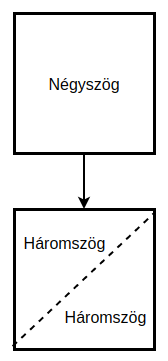
\includegraphics[scale=0.39]{images/triangulation.png}
\caption{Háromszögesítés elémletben.}
\label{fig:tri}
\end{figure}

\noindent A célünk ezzel, a \ref{fig:tri}. ábrán  látható módon minden négyszög síkodomot felbontsunk két különböző háromszögre szaggatott vonalon való metszéssel. Persze az ábrán látható négyszög egy szabályos négyzet, de ezek a négyszögek felvehetnek többféle alakzatot (téglalap, deltoid, rombusz stb...).\\

Ez úgy valósul meg, hogy a program kiválasztja az első beolvasott négyszöget az OBJ fájlból annak első három csúcs koordinátájából képez egy háromszöget majd a következő háromszöget az előző négyszög első harmadik illetve negyedik koordinátájából képezi le, így végighaladva az összes négyszögön ami az OBJ fájlunkban található.\\Ennek szemléletetése a \ref{fig:tri1}. ábrán látható.
\begin{figure}[h]
\centering
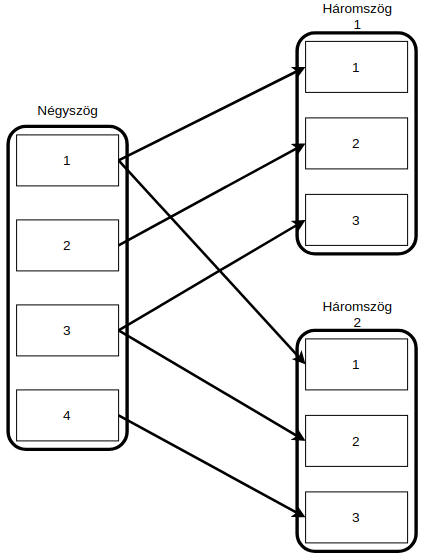
\includegraphics[scale=0.39]{images/haromszog.png}
\caption{Háromszögesítés diagram.}
\label{fig:tri1}
\end{figure}

Megvalósítás során \texttt{triangulation\_of\_quads} funkció modell struktúránkból elveszi az összes négyszöget és két háromszöggel tölti fel azok helyét, illetve a lapok számát is növeli minden felvágott négyszög esetében eggyel.

\begin{figure}[h]
\centering
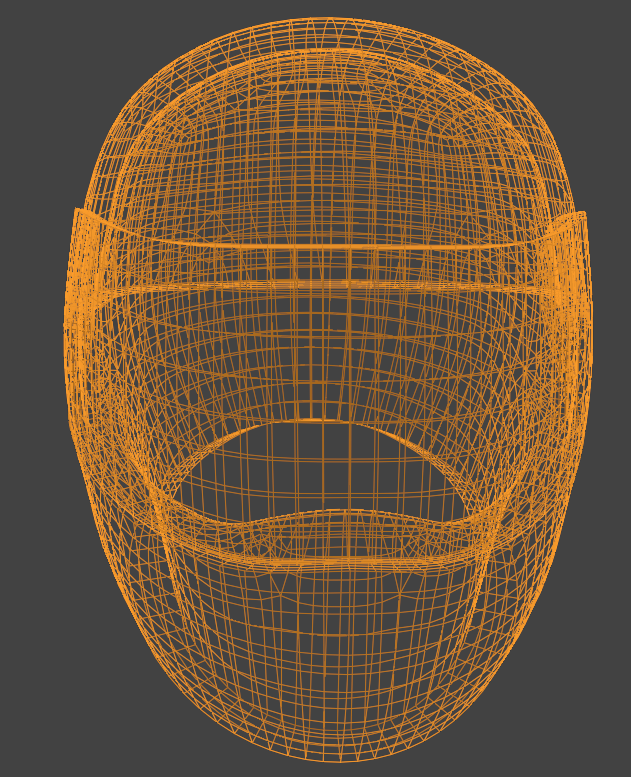
\includegraphics[scale=0.32]{images/helmet1.png}
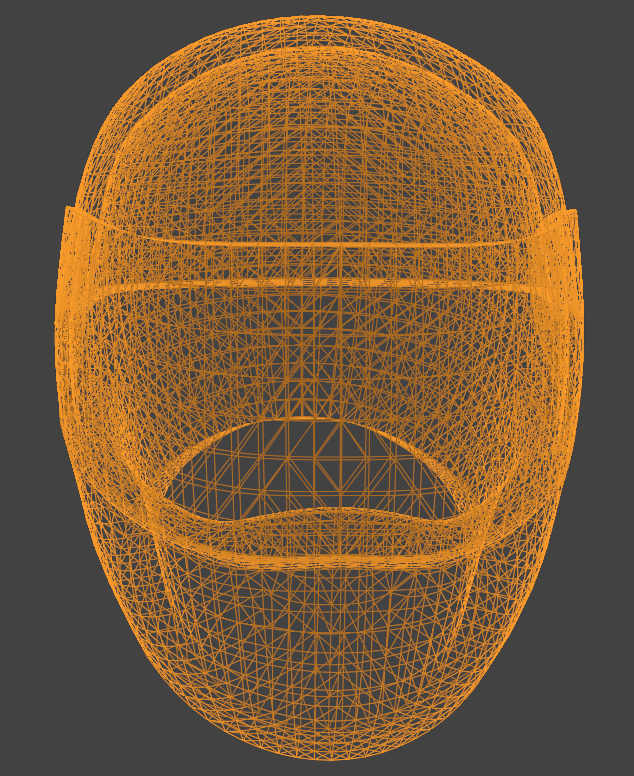
\includegraphics[scale=0.32]{images/helmet2.png}
\caption{helmet.obj háló.}
\label{fig:tri2}
\end{figure}

Az \ref{fig:tri2}. ábra bal oldali képen az eredeti \texttt{helmet.obj} modell látható, a modell hálójának megjelenítésével, a jobb oldali képen pedig már a háromszögelt változat. Jól láthatóak az eltérések a két modell rajzolt állapota között.
\begin{table}[h]
\centering
\caption{helmet.obj adatait tartalmazó táblázat}
\bigskip
\label{tab:modellek}
\begin{tabular}{l|c|c|}
& helmet.obj & helmet.obj háromszögesítés után \\
\hline
geometria vektorok & 6066 & 6066 \\
textúra koordináták & 6409 & 6409 \\
normál vektorok & 6650 & 6650 \\
arc elemek & 6064 & 12128 \\
háromszögek & 0 & 12128 \\
négyszögek & 6064 & 0 \\
\hline
\end{tabular}
\label{fig:tri3}
\end{table}

Az \ref{fig:tri3}. összesítő táblázat megmutatja hogyan változtak a \texttt{helmet.obj} adatai a háromszögesítés után. Láthatóan az összes négyszög eltünt a modellből ezeket két háromszögre bontotta a szoftver, az arc elemek száma is duplájára nőtt.
\newpage
\SubSection{Bejárási irány megváltoztatás}
\bigskip
A program ezen része arra szolgál, hogy a háromszögeink bejárási irányát meg tudjuk változtatni \aref{fig:bej1}. ábrán látható módon.
\bigskip
\begin{figure}[h]
\centering
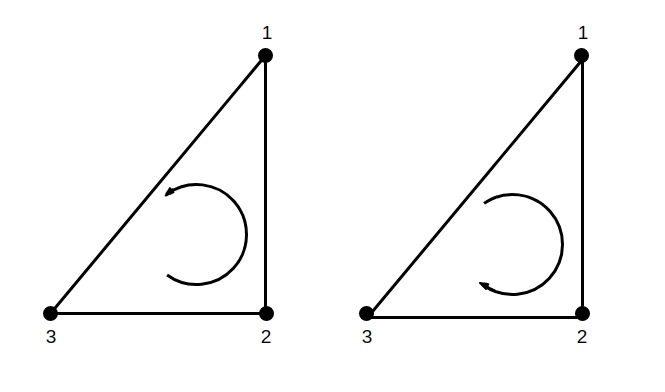
\includegraphics[scale=0.5]{images/bejarasi.png}
\caption{Bejárási irány változtatás elméletben.}
\label{fig:bej1}
\end{figure}
\bigskip

Egy háromszög csúcsok közötti bejárást kétféleképpen tudjuk bejárni. \Aref{fig:bej1}. ábrán bal oldalt látható  óramutató járásával ellentétes bejárási sorrendben (1 -> 3 -> 2), amit a glut alapból használ, jobb oldalon pedig az ellenkezője óramutató járásával megegyező bejárás (1 -> 2 -> 3).\\

Ez a funkció \texttt{change\_vertex\_order} függvény néven van a programba implementálva. Amennyiben úgy döntünk és ezt alkalmazzuk a programunk elvégzi a bejárási irány cserét model struktúrába betöltött objektomunkon.\\

Megjelenítés során a megjelenítő ugyanúgy óramutatójárásval ellentétesen fogja megjeleníteni a modellünket, viszont a programunk \texttt{change\_vertex\_order} függvény segítségével megváltoztatta csúcsok sorrendjét így a megjelenítés már óramutató járásával megegyező módon fog történni az eredeti OBJ fájlhoz képest.\\
\newpage
\Aref{fig:bej2}. ábra egy egyszerű modellen keresztül ezt hivatott bemutatni.
\bigskip
\begin{figure}[h]
\centering
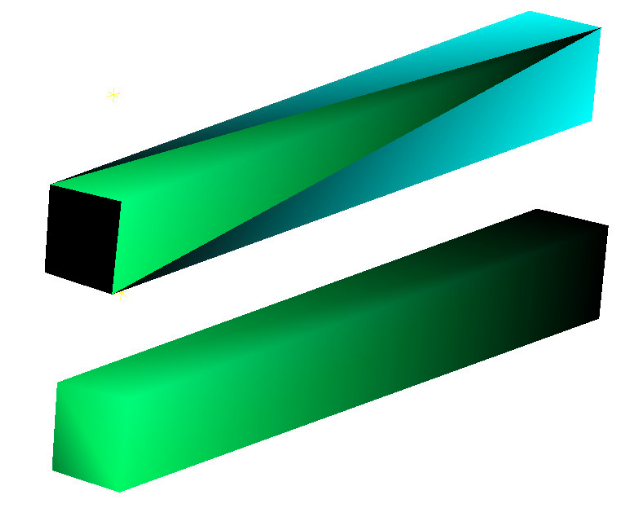
\includegraphics[scale=0.5]{images/order.png}
\caption{Bejárási irány hiba.}
\label{fig:bej2}
\end{figure}
\bigskip

Jól látható módon a felső modellünk hibás az alsó pedig jól került megjelenítésre. Két modell összesen az arcok közötti bejárási útvonal a különbség a két modell összes többi vektora ugyanaz \aref{fig:bej3} táblázatban bemutatásra kerül a két objektum közti eltérés. Ez a táblázat csak az arcok közötti eltérést mutatja.

\newpage

\begin{table}[h]
\centering
\caption{Arc elemeket összehasonlító táblázat}
\bigskip
\begin{tabular}{|c|c|}
Felső modell& Alsó modell \\
\hline
f  1//1 2//2 3//3 & f  1//1 3//3 2//2 \\
f  1//1 3//3 4//4 & f  1//1 4//4 3//3 \\
f  5//5 6//6 7//7 & f  5//5 7//7 6//6 \\
f  5//5 7//7 8//8 & f  5//5 8//8 7//7 \\ 
f  1//1 2//2 6//6 & f  1//1 6//6 2//2 \\
f  1//1 5//5 6//6 & f  1//1 6//6 5//5 \\
f  1//1 4//4 8//8 & f  1//1 8//8 4//4 \\
f  1//1 5//5 8//8 & f  1//1 8//8 5//5 \\
f  3//3 6//6 7//7 & f  3//3 7//7 6//6 \\
f  2//2 3//3 6//6 & f  2//2 6//6 3//3 \\
f  3//3 8//8 7//7 & f  3//3 7//7 8//8 \\
f  3//3 4//4 8//8 & f  3//3 8//8 4//4 \\
\hline
\end{tabular}
\label{fig:bej3}
\end{table}
\bigskip 

\Aref{fig:bej3} táblázatból láthatóan kivehető, hogy a háromszögünk arcfelsorolás iránya megváltozott a második és harmadik koordinátán, ezáltal a megjelenítés óramutató járásával megegyezően fog történni az eredeti OBJ fájl-hoz képest.

\Section {Fájlba írás}
Változtatott OBJ fájl kiírása \texttt{obj\_output.obj} fájlba \texttt{write\_to\_file} függvény segítségével kivitelezhető. OBJ fájlunk betöltése és az elvégzett változtatások után a program megkérdezi kívánjuk menteni a változtatott OBJ fájlt, amennyiben így döntünk a program létrehozza az \texttt{obj\_output.obj} fájlt és azt feltölti model struktúránk aktuális adataival. A mentett fájlunkba kiírt OBJ fájl nem tartalmazza a betöltött fájl anyagjellemzőit illetve a megjegyzéseit sem.
\bigskip
\dirtree{%
.1 /obj\_corrector\_tool.
.2 /include.
.2 /OBJ.
.2 /src.
.2 /tests.
.2 /Makefile.
.2 /obj\_output.obj.
}
\bigskip

Ez a kimeneti fájl közvetlen az \texttt{obj\_corrector\_tool} könyvtárba kerül eltárolásra a program futtatása után.






